\documentclass[a4paper,12pt]{article}

\usepackage[utf8]{inputenc}
\usepackage[spanish]{babel}
\usepackage[margin=1cm, top=1cm, includefoot]{geometry}
\usepackage{graphicx}
\usepackage{xcolor}
\usepackage{enumitem}  % opcional, para mejor control de listas
\usepackage[most]{tcolorbox}% Para la insercion de cuadros en la portada
\usepackage[export]{adjustbox}

% Color de fondo solo en la portada
\definecolor{grisplomo}{rgb}{0.95, 0.95, 0.95}

% Color verde HackTheBox
\definecolor{greenPortada}{HTML}{69A84F}

% Variables
\newcommand{\logoPortada}{Images/hackthebox_logo.png}
\newcommand{\machineName}{Reversing :: IronHeartEcho}

\begin{document}

% === PORTADA CON COLOR DE FONDO ===
{\pagecolor{grisplomo}
\begin{titlepage}
    \centering
    \includegraphics[width=\textwidth]{\logoPortada}\par
    \vspace{0.5cm}

    {\scshape\LARGE \textbf{Neurogrid CTF: Human-Only}\par}
    \vspace{0.5cm}

    {\Huge\bfseries\textcolor{greenPortada}{\machineName}\par}
    \vspace{0.5cm}

    {\LARGE
    \begin{enumerate}[leftmargin=*,label=\textbf{\arabic*.},itemsep=0.2em]
        \item Quick view of the downloaded file:\\
              \texttt{:  ls -l ./rev\_ironheart\_echo.zip}

        \item We decompress in silent mode:\\
              \texttt{:  unzip -q ./rev\_ironheart\_echo.zip}

        \item We display the structure and enter the folder:\\
              \texttt{:  tree \&\& cd ./rev\_ironheart\_echo}

							\begin{adjustbox}{max width=\paperwidth,center}
              \vspace{0.6cm}
              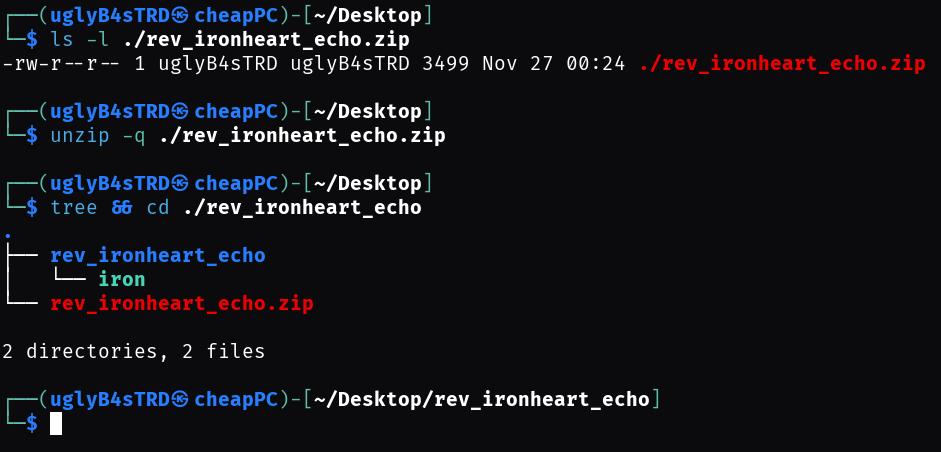
\includegraphics[width=1\textwidth]{Images/step_01.png}
              \vspace{1cm}
							\end{adjustbox}

				\par\vspace{4cm}
        \item Run and test the binary:\\
              \texttt{:  ./iron}

        \item \textbf{ltrace} 'It is useful for debugging/understanding a binary without having its source code':\\
              \texttt{:  ltrace ./iron}

        \item Our input \texttt{TeSt\_string\_HERE} is compared with \texttt{strcmp()},\\
              we find the flag in the second argument...!!!\\    "HTB\{r3wr1tt3n\_r3s0nanc3\}" 

							\begin{adjustbox}{max width=\paperwidth,center}
              \vspace{0.6cm}
              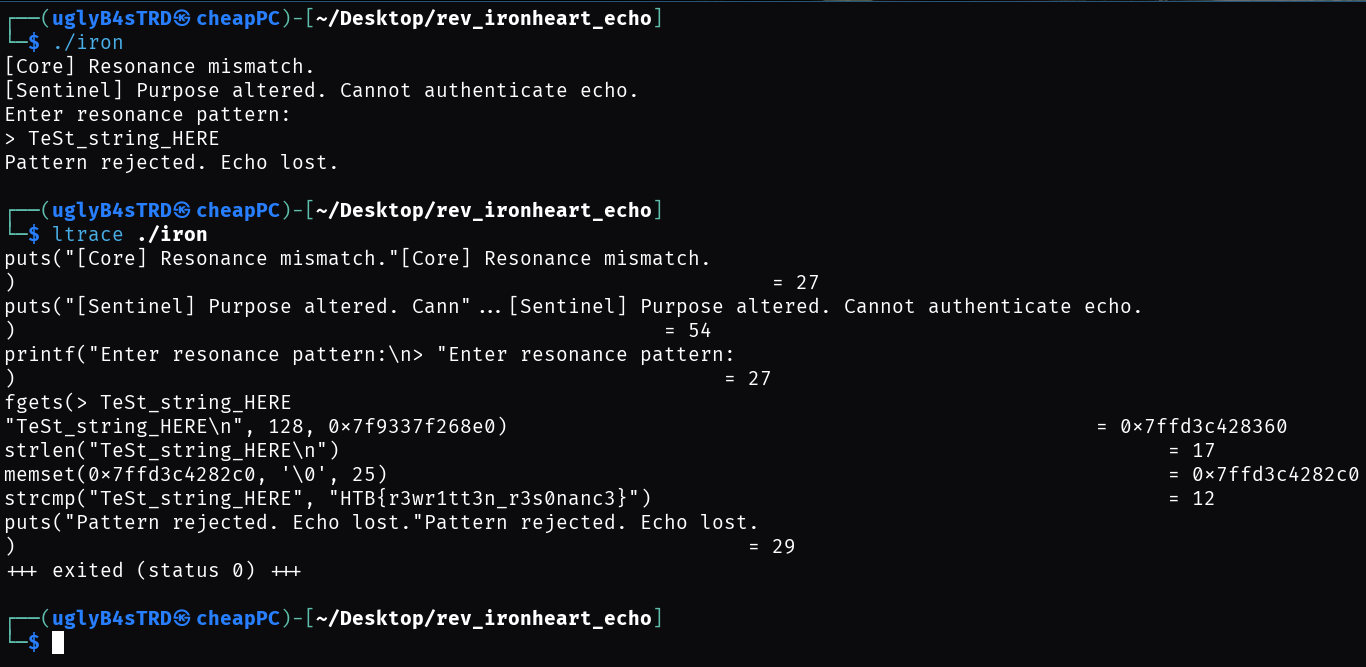
\includegraphics[width=1\textwidth]{Images/step_02.png}
              \vspace{0.8cm}
							\end{adjustbox}
    \end{enumerate}
    }

    \vfill
		\begin{tcolorbox}[colback=red!5!white,colframe=red!75!black]
			\centering
			{\small \textit{WriteUp by x89p}}
		\end{tcolorbox}
\end{titlepage}

\end{document}
